\documentclass[12pt,a4paper]{article}

% =========================
% PACOTES
% =========================
\usepackage[T1]{fontenc}
\usepackage[utf8]{inputenc}
\usepackage[brazil]{babel}
\usepackage{amsmath,amssymb}
\usepackage[a4paper,top=3cm,bottom=2.5cm,left=3cm,right=2cm]{geometry}
\usepackage{graphicx}
\usepackage{fancyhdr}
\usepackage{float}
\usepackage{setspace}
\usepackage{indentfirst}
\usepackage{pgfplots}
\usepackage{tikz}
\usepackage[american]{circuitikz}
\usepackage{lmodern}
\usepackage{tocloft}
\usepackage{array}
\usepackage{lastpage}
\usepackage{xcolor}
\usepackage[most]{tcolorbox}
\usepackage{graphicx}
\usepackage{float}

% =========================
% CAIXAS PARA CÁLCULOS
% =========================
\newtcolorbox{calcbox}[1][]{
    enhanced,
    breakable,
    colback=gray!3,
    colframe=black!70,
    boxrule=0.6pt,
    arc=2mm,
    left=8pt,
    right=8pt,
    top=8pt,
    bottom=8pt,
    before skip=10pt,
    after skip=10pt,
    title=#1,
    fonttitle=\bfseries,
    colbacktitle=gray!12,
    coltitle=black
}

\tcbset{
    calculoestilo/.style={
        breakable,
        enhanced,
        colback=gray!3,
        colframe=black!65,
        boxrule=0.5pt,
        arc=2mm,
        left=8pt,
        right=8pt,
        top=8pt,
        bottom=8pt,
        fonttitle=\bfseries,
        coltitle=black,
        colbacktitle=gray!12,
        attach boxed title to top left={xshift=4mm,yshift=-2mm},
        boxed title style={
            colframe=black!65,
            colback=gray!12,
            boxrule=0.5pt,
            arc=1mm
        }
    }
}

% =========================
% CONFIGURAÇÕES GERAIS
% =========================
\pgfplotsset{compat=1.18}
\onehalfspacing

% =========================
% CONFIGURAÇÕES DA PÁGINA
% =========================
\geometry{top=2.8cm,bottom=2.8cm,left=3cm,right=2.5cm}
\onehalfspacing
\setlength{\parindent}{1.25cm}
\setlength{\headheight}{45pt}
\setlength{\footskip}{28pt}

% =========================
% COMANDO PARA ESPAÇO DE FOTO
% =========================
\newcommand{\EspacoFoto}[2]{
\begin{figure}[H]
\centering
\fbox{
    \begin{minipage}[c][#1][c]{0.88\textwidth}
        \centering
        {\large #2}

        \vfill
        \textit{Inserir fotografia ou imagem nesta área.}
        \vfill
    \end{minipage}
}
\end{figure}
}

% =========================
% CABEÇALHO E RODAPÉ
% =========================
\pagestyle{fancy}
\fancyhf{}
\fancyhead[L]{
\includegraphics[height=1.3cm]{logo-ifmt.png}}
\fancyhead[R]{\small Circuitos Elétricos II\\ \small Relatório Técnico Acadêmico}
\fancyfoot[C]{\fontsize{8.5}{10}\selectfont Instituto Federal de Educação, Ciência e Tecnologia de Mato Grosso -- IFMT \;|\; Página \thepage\ de \pageref{LastPage}}
\renewcommand{\headrulewidth}{0.4pt}
\renewcommand{\footrulewidth}{0.4pt}

% =========================
% INÍCIO DO DOCUMENTO
% =========================
\begin{document}
%==================================================
% CAPA
%==================================================
\begin{titlepage}
\thispagestyle{empty}

\begin{center}

\vspace*{2cm}


\includegraphics[width=1.0\textwidth]{logo-ifmt.png}

\vspace{1.2cm}

{\normalsize \textbf{INSTITUTO FEDERAL DE EDUCAÇÃO, CIÊNCIA E TECNOLOGIA DE MATO GROSSO}}\\[0.2cm]
{\normalsize Campus Pontes e Lacerda -- Fronteira Oeste}

\vspace{3.5cm}


{\large Nicoly Canteiro Araújo e colegas de grupo}\\



\vfill

{\Large \textbf{RELATÓRIO TÉCNICO}}\\[0.4cm]
{\large \textbf{EXPERIMENTO II}}\\[0.8cm]
{\large Análise teórica e experimental da carga e descarga de capacitor em circuito RC de primeira ordem}

\vfill

Pontes e Lacerda -- MT\\
2026

\end{center}
\end{titlepage}

%==================================================
% FOLHA DE ROSTO
%==================================================
\begin{titlepage}
\thispagestyle{empty}

\begin{center}

\vspace*{2cm}

{\large Nicoly Canteiro Araújo e colegas de grupo}\\


\vspace{4cm}

{\Large \textbf{RELATÓRIO TÉCNICO}}\\[0.4cm]
{\large \textbf{EXPERIMENTO II}}\\[0.8cm]
{\large Análise teórica e experimental da carga e descarga de capacitor em circuito RC de primeira ordem}

\end{center}

\vspace{2.5cm}

\hfill
\begin{minipage}{0.48\textwidth}
\singlespacing
Relatório técnico apresentado ao Instituto Federal de Educação, Ciência e Tecnologia de Mato Grosso -- Campus Pontes e Lacerda -- Fronteira Oeste, como requisito parcial para avaliação na disciplina de Circuitos Elétricos II.

\vspace{0.8cm}

\textbf{Professor(a):} Professor da disciplina\\
\textbf{Disciplina:} Circuitos Elétricos II\\
\textbf{Curso:} Bacharelado em Engenharia Elétrica
\end{minipage}

\vfill

\begin{center}
Pontes e Lacerda -- MT\\
2026
\end{center}

\end{titlepage}
% =========================
% RESUMO
% =========================
\section*{Resumo}

Este relatório técnico apresenta a análise teórica e experimental do comportamento de carga e descarga de um capacitor em um circuito RC de primeira ordem. O estudo teve como finalidade determinar as constantes de tempo do circuito, comparar os resultados experimentais com o modelo exponencial previsto teoricamente e representar graficamente a variação da tensão no capacitor ao longo do tempo. A partir dos parâmetros fornecidos, foram desenvolvidos os cálculos teóricos, organizadas tabelas de resultados e elaborado um gráfico representativo do processo transitório. Os resultados obtidos mostram compatibilidade com a teoria dos circuitos de primeira ordem, evidenciando a influência da resistência equivalente sobre a dinâmica de carga e descarga do capacitor.

\newpage

% =========================
% SUMÁRIO
% =========================
\tableofcontents
\newpage

% =========================
\section{Objetivos}

O presente experimento teve como objetivos principais:

\begin{itemize}
    \item analisar o processo de carga e descarga de um capacitor;
    \item determinar as constantes de tempo do circuito;
    \item comparar os resultados experimentais com os valores teóricos;
    \item observar o comportamento transitório da tensão no capacitor;
    \item representar graficamente a resposta temporal do circuito RC.
\end{itemize}

% =========================
\section{Materiais e Parâmetros do Circuito}

Para a realização do experimento, foram considerados os seguintes parâmetros:

\begin{itemize}
    \item fonte de tensão contínua: $E = 10\,V$;
    \item resistor $R_1 = 1\,k\Omega$;
    \item resistor $R_2 = 1\,k\Omega$;
    \item capacitor $C = 100\,\mu F = 100 \times 10^{-6}\,F$;
    \item chave seletora de três posições.
\end{itemize}

% =========================
\section{Circuito Analisado}

A Figura \ref{fig:circuito_rc} apresenta o circuito RC utilizado na análise.

\begin{figure}[H]
    \centering
    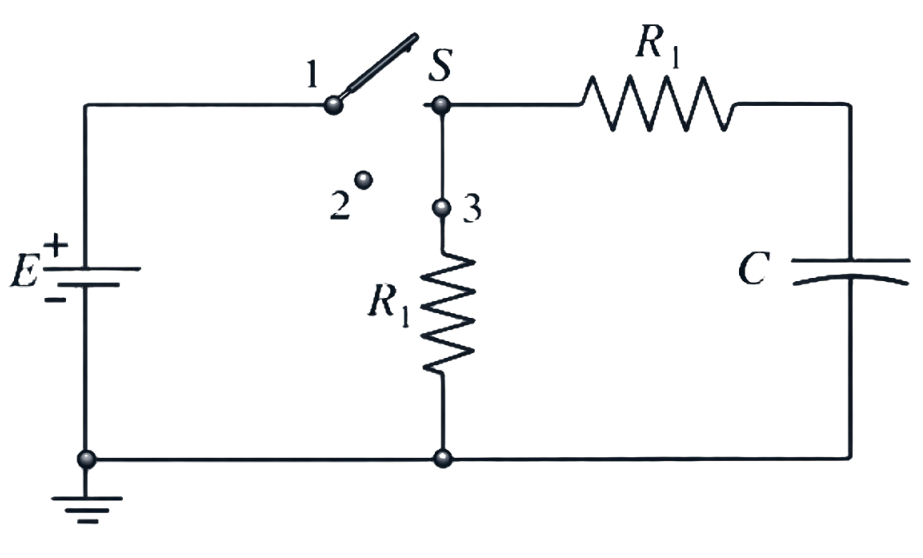
\includegraphics[width=0.9\textwidth]{circuitoRC.png}
    \caption{Circuito elétrico RC.}
    \label{fig:circuito_rc}
\end{figure}

% =========================
\section{Fundamentação Teórica}

Em circuitos RC de primeira ordem, a tensão no capacitor varia de forma exponencial com o tempo.

\begin{calcbox}[Equação da carga]
Durante a carga, a tensão no capacitor é descrita por:
\[
V_C(t)=V\left(1-e^{-t/\tau}\right)
\]
\end{calcbox}

\begin{calcbox}[Equação da descarga]
Durante a descarga, a expressão correspondente é:
\[
V_C(t)=V_0e^{-t/\tau}
\]
\end{calcbox}

\begin{calcbox}[Constante de tempo]
A constante de tempo do circuito é definida por:
\[
\tau = RC
\]
\end{calcbox}

A constante de tempo indica a rapidez da resposta transitória do circuito. \\ Após aproximadamente $5\tau$, considera-se que o sistema atingiu regime permanente.

\newpage
% =========================
\section{Cálculos Resolvidos}

\subsection{Constante de tempo na carga}

Durante a carga, o capacitor está associado apenas à resistência $R_1$.

\begin{calcbox}[Determinação de $\tau_1$]
\[
\tau_1 = R_1C
\]

Substituindo os valores:

\[
\tau_1 = (1000)(100 \times 10^{-6})
\]

\[
\tau_1 = 1000 \times 0{,}0001
\]

\[
\tau_1 = 0{,}1\,s
\]

Logo:

\[
\tau_1 = 100\,ms
\]
\end{calcbox}

\begin{calcbox}[Equação teórica da carga]
\[
V_C(t)=10\left(1-e^{-t/0{,}1}\right)
\]
\end{calcbox}

\subsection{Resistência equivalente na descarga}

Durante a descarga, a corrente percorre $R_1$ e $R_2$.

\begin{calcbox}[Determinação da resistência equivalente]
\[
R_{eq}=R_1+R_2
\]

\[
R_{eq}=1\,k\Omega + 1\,k\Omega
\]

\[
R_{eq}=2\,k\Omega
\]
\end{calcbox}

\subsection{Constante de tempo na descarga}

\begin{calcbox}[Determinação de $\tau_2$]
\[
\tau_2 = R_{eq}C
\]

\[
\tau_2 = (2000)(100 \times 10^{-6})
\]

\[
\tau_2 = 2000 \times 0{,}0001
\]

\[
\tau_2 = 0{,}2\,s
\]

Logo:

\[
\tau_2 = 200\,ms
\]
\end{calcbox}

\begin{calcbox}[Equação teórica da descarga]
\[
V_C(t)=10e^{-t/0{,}2}
\]
\end{calcbox}

\newpage
\subsection{Exemplo resolvido da carga}

Para o instante de $t = 500\,ms$, considerando o início da carga em $400\,ms$:

\begin{calcbox}[Cálculo da tensão na carga]
\[
t' = 500 - 400 = 100\,ms = 0{,}1\,s
\]

Como $\tau_1 = 0{,}1\,s$:

\[
\frac{t'}{\tau_1} = \frac{0{,}1}{0{,}1}=1
\]

Substituindo na equação:

\[
V_C(t)=10(1-e^{-1})
\]

Como $e^{-1} \approx 0{,}3679$:

\[
V_C(t)=10(1-0{,}3679)
\]

\[
V_C(t)=10(0{,}6321)
\]

\[
V_C(t)\approx 6{,}32\,V
\]
\end{calcbox}

\newpage
\subsection{Exemplo resolvido da descarga}

Para o instante de $t = 1380\,ms$, considerando o início da descarga em $1180\,ms$:

\begin{calcbox}[Cálculo da tensão na descarga]
\[
t' = 1380 - 1180 = 200\,ms = 0{,}2\,s
\]

Como $\tau_2 = 0{,}2\,s$:

\[
\frac{t'}{\tau_2} = \frac{0{,}2}{0{,}2}=1
\]

Substituindo na equação:

\[
V_C(t)=10e^{-1}
\]

\[
V_C(t)=10(0{,}3679)
\]

\[
V_C(t)\approx 3{,}68\,V
\]
\end{calcbox}

\newpage
% =========================
\section{Resultados Experimentais}

\subsection{Carga do capacitor}

Para a etapa de carga, considerou-se o instante inicial em $400\,ms$. Assim, o tempo normalizado foi calculado por:

\begin{calcbox}[Normalização do tempo na carga]
\[
\frac{t'}{\tau_1}=\frac{t-400}{100}
\]
\end{calcbox}

\begin{table}[H]
\centering
\caption{Dados experimentais e teóricos da carga do capacitor.}
\begin{tabular}{|c|c|c|c|}
\hline
Tempo (ms) & $t'/\tau_1$ & Tensão experimental (V) & Tensão teórica (V) \\
\hline
400 & 0.0 & 0.00 & 0.00 \\
420 & 0.2 & 1.60 & 1.81 \\
440 & 0.4 & 3.00 & 3.30 \\
460 & 0.6 & 4.20 & 4.51 \\
480 & 0.8 & 5.00 & 5.51 \\
500 & 1.0 & 5.60 & 6.32 \\
520 & 1.2 & 6.40 & 6.99 \\
540 & 1.4 & 6.80 & 7.53 \\
560 & 1.6 & 7.20 & 7.98 \\
580 & 1.8 & 7.60 & 8.35 \\
600 & 2.0 & 8.20 & 8.65 \\
620 & 2.2 & 8.40 & 8.89 \\
640 & 2.4 & 8.60 & 9.09 \\
660 & 2.6 & 8.80 & 9.26 \\
700 & 3.0 & 9.00 & 9.50 \\
\hline
\end{tabular}
\end{table}

\newpage
\subsection{Descarga do capacitor}

Para a etapa de descarga, considerou-se o instante inicial em $1180\,ms$. Assim, o tempo normalizado foi calculado por:

\begin{calcbox}[Normalização do tempo na descarga]
\[
\frac{t'}{\tau_2}=\frac{t-1180}{200}
\]
\end{calcbox}

\begin{table}[H]
\centering
\caption{Dados experimentais e teóricos da descarga do capacitor.}
\begin{tabular}{|c|c|c|c|}
\hline
Tempo (ms) & $t'/\tau_2$ & Tensão experimental (V) & Tensão teórica (V) \\
\hline
1180 & 0.0 & 9.20 & 10.00 \\
1200 & 0.1 & 8.20 & 9.05 \\
1220 & 0.2 & 8.40 & 8.19 \\
1240 & 0.3 & 7.40 & 7.41 \\
1260 & 0.4 & 7.02 & 6.70 \\
1300 & 0.6 & 6.40 & 5.49 \\
1320 & 0.7 & 5.40 & 4.97 \\
1340 & 0.8 & 5.00 & 4.49 \\
1380 & 1.0 & 4.60 & 3.68 \\
1400 & 1.1 & 4.00 & 3.33 \\
\hline
\end{tabular}
\end{table}

\newpage
% =========================
\section{Análise Gráfica da Carga e Descarga do Capacitor}

O comportamento transitório do capacitor pode ser analisado por meio de duas representações gráficas: uma apresentação acadêmica convencional, adequada para comparação entre valores teóricos e experimentais, e uma apresentação complementar em estilo osciloscópio, que permite visualização mais intuitiva da dinâmica de carga e descarga ao longo do tempo.
\\

\begin{figure}[H]
\centering
\begin{tikzpicture}
\begin{axis}[
    width=15cm,
    height=9cm,
    xlabel={Tempo relativo (ms)},
    ylabel={Tensão no capacitor (V)},
    xmin=0, xmax=300,
    ymin=0, ymax=10.5,
    grid=major,
    legend style={at={(0.5,-0.2)}, anchor=north, legend columns=2},
    title={Comportamento de carga e descarga do capacitor}
]

\addplot[
    only marks,
    mark=*
] coordinates {
    (0,0.00)
    (20,1.60)
    (40,3.00)
    (60,4.20)
    (80,5.00)
    (100,5.60)
    (120,6.40)
    (140,6.80)
    (160,7.20)
    (180,7.60)
    (200,8.20)
    (220,8.40)
    (240,8.60)
    (260,8.80)
    (300,9.00)
};

\addplot[
    domain=0:300,
    samples=200,
    thick
] {10*(1-exp(-x/100))};

\addplot[
    only marks,
    mark=square*
] coordinates {
    (0,9.20)
    (20,8.20)
    (40,8.40)
    (60,7.40)
    (80,7.02)
    (120,6.40)
    (140,5.40)
    (160,5.00)
    (200,4.60)
    (220,4.00)
};

\addplot[
    domain=0:220,
    samples=200,
    thick,
    dashed
] {10*exp(-x/200)};

\legend{Carga experimental, Carga teórica, Descarga experimental, Descarga teórica}

\end{axis}
\end{tikzpicture}
\caption{Curvas de carga e descarga do capacitor.}
\end{figure}

\subsection{Gráfico complementar com estrutura visual estilo osciloscópio}

\begin{figure}[H]
\centering
\begin{tikzpicture}

% Painel externo do "osciloscópio"
\node[
    rounded corners=6pt,
    fill=black!94,
    draw=black!70,
    minimum width=16.8cm,
    minimum height=10.8cm,
    inner sep=0pt
] (panel) {};

% Eixo do gráfico centralizado no painel
\begin{axis}[
    at={(panel.center)},
    anchor=center,
    width=13.9cm,
    height=7.6cm,
    scale only axis,
    xmin=0, xmax=300,
    ymin=0, ymax=10.5,
    xtick={0,20,...,300},
    ytick={0,2,...,10},
    minor x tick num=1,
    minor y tick num=1,
    xlabel={Tempo relativo (ms)},
    ylabel={Tensão no capacitor (V)},
    title={Comportamento de carga e descarga do capacitor},
    xlabel style={color=white, font=\normalsize},
    ylabel style={color=white, font=\normalsize},
    title style={color=white, font=\bfseries\normalsize, yshift=4pt},
    tick label style={color=white, font=\small},
    tick style={color=green!70!white},
    axis line style={color=green!70!white, line width=0.8pt},
    axis background/.style={fill=black!97},
    grid=major,
    major grid style={draw=green!45!black, line width=0.45pt},
    minor grid style={draw=green!25!black, line width=0.2pt},
    legend style={
        at={(0.5,-0.20)},
        anchor=north,
        legend columns=2,
        fill=black!95,
        draw=green!70!white,
        text=white,
        font=\small
    },
    legend cell align=left
]

% -------------------------------------------------
% CARGA TEÓRICA - brilho + curva principal
% -------------------------------------------------
\addplot[
    domain=0:300,
    samples=300,
    line width=4pt,
    color=cyan!30,
    opacity=0.30
] {10*(1-exp(-x/100))};

\addplot[
    domain=0:300,
    samples=300,
    line width=1.4pt,
    color=cyan!95
] {10*(1-exp(-x/100))};

% -------------------------------------------------
% DESCARGA TEÓRICA - brilho + curva principal
% -------------------------------------------------
\addplot[
    domain=0:220,
    samples=300,
    line width=4pt,
    color=orange!40,
    opacity=0.25,
    dashed
] {10*exp(-x/200)};

\addplot[
    domain=0:220,
    samples=300,
    line width=1.4pt,
    color=orange!95,
    dashed
] {10*exp(-x/200)};

% -------------------------------------------------
% CARGA EXPERIMENTAL
% -------------------------------------------------
\addplot[
    only marks,
    mark=*,
    mark size=2.1pt,
    color=yellow!95,
    mark options={fill=yellow!95, draw=yellow!20!white}
] coordinates {
    (0,0.00)
    (20,1.60)
    (40,3.00)
    (60,4.20)
    (80,5.00)
    (100,5.60)
    (120,6.40)
    (140,6.80)
    (160,7.20)
    (180,7.60)
    (200,8.20)
    (220,8.40)
    (240,8.60)
    (260,8.80)
    (300,9.00)
};

% -------------------------------------------------
% DESCARGA EXPERIMENTAL
% -------------------------------------------------
\addplot[
    only marks,
    mark=square*,
    mark size=2.1pt,
    color=lime!85!white,
    mark options={fill=lime!85!white, draw=lime!20!white}
] coordinates {
    (0,9.20)
    (20,8.20)
    (40,8.40)
    (60,7.40)
    (80,7.02)
    (120,6.40)
    (140,5.40)
    (160,5.00)
    (200,4.60)
    (220,4.00)
};

% -------------------------------------------------
% LINHAS DE REFERÊNCIA DAS CONSTANTES DE TEMPO
% -------------------------------------------------
\addplot[white!70, densely dotted, line width=0.7pt] coordinates {(100,0) (100,6.32)};
\addplot[white!70, densely dotted, line width=0.7pt] coordinates {(0,6.32) (100,6.32)};

\addplot[white!70, densely dotted, line width=0.7pt] coordinates {(200,0) (200,3.68)};
\addplot[white!70, densely dotted, line width=0.7pt] coordinates {(0,3.68) (200,3.68)};

% -------------------------------------------------
% ANOTAÇÕES VISUAIS
% -------------------------------------------------
\node[
    fill=black!88,
    draw=cyan!80,
    text=white,
    rounded corners=2pt,
    inner sep=2pt,
    font=\scriptsize
] at (axis cs:220,9.25) {Carga teórica};

\node[
    fill=black!88,
    draw=orange!90,
    text=white,
    rounded corners=2pt,
    inner sep=2pt,
    font=\scriptsize
] at (axis cs:150,2.10) {Descarga teórica};

\node[
    fill=black!88,
    draw=blue!60,
    text=white,
    rounded corners=2pt,
    inner sep=2pt,
    font=\scriptsize
] at (axis cs:82,7.00) {$\tau_{\text{carga}}=100\,ms$};

\node[
    fill=black!88,
    draw=red!70,
    text=white,
    rounded corners=2pt,
    inner sep=2pt,
    font=\scriptsize
] at (axis cs:225,4.20) {$\tau_{\text{descarga}}=200\,ms$};

\legend{
Carga teórica,
Descarga teórica,
Carga experimental,
Descarga experimental
}

\end{axis}

\end{tikzpicture}
\caption{Gráfico complementar em estilo osciloscópio, com identificação completa dos eixos, malha visual e representação das curvas teóricas e experimentais da carga e descarga do capacitor.}
\label{fig:grafico_osciloscopio_estruturado}
\end{figure}

\newpage
% =========================
\section{Discussão}

Os resultados obtidos apresentaram comportamento compatível com a resposta transitória de um circuito RC de primeira ordem. Durante a carga, observou-se aumento gradual da tensão no capacitor até sua aproximação ao valor da fonte, enquanto, na descarga, verificou-se decaimento progressivo da tensão armazenada, conforme previsto pelo modelo exponencial teórico.

A realização do experimento demandou duas visitas técnicas ao Laboratório de Eletrônica, uma vez que foram necessárias tentativas sucessivas para a montagem do circuito e para a correta observação dos processos de carga e descarga do capacitor. Essas visitas contribuíram para a obtenção dos dados experimentais e para a verificação prática do comportamento do circuito.

Além disso, verificou-se que a descarga ocorreu de forma mais lenta do que a carga, em razão da maior resistência equivalente associada a essa etapa, o que resultou em constante de tempo superior. As pequenas diferenças entre os valores teóricos e experimentais podem ser atribuídas à tolerância dos componentes, ao tempo de comutação da chave e às limitações dos instrumentos de medição.

% =========================
\section{Conclusão}

A análise permitiu compreender o comportamento de carga e descarga de um capacitor em circuito RC de primeira ordem, possibilitando a determinação das constantes de tempo e a comparação entre os resultados experimentais e teóricos. Verificou-se que a tensão no capacitor varia exponencialmente, conforme previsto pela teoria, e que a resistência equivalente exerce influência direta sobre a resposta temporal do sistema.

Dessa forma, conclui-se que o experimento atingiu os objetivos propostos, contribuindo para a consolidação prática dos conceitos de circuitos transitórios de primeira ordem.

\newpage
% =========================
\section{Documentação Fotográfica da Montagem Experimental}

\begin{figure}[H]
    \centering
    \fbox{\parbox{0.7\textwidth}{\centering\vspace{1cm}Foto do experimento omitida nesta versão pública\vspace{1cm}}}
    \caption{Montagem inicial do circuito em protoboard para a realização do experimento.}
    \label{fig:foto01}
\end{figure}

\begin{figure}[H]
    \centering
    \fbox{\parbox{0.7\textwidth}{\centering\vspace{1cm}Foto do experimento omitida nesta versão pública\vspace{1cm}}}
    \caption{Remontagem do circuito na segunda etapa experimental, realizada no Laboratório de Eletrônica.}
    \label{fig:foto02}
\end{figure}

\begin{figure}[H]
    \centering
    \fbox{\parbox{0.7\textwidth}{\centering\vspace{1cm}Foto do experimento omitida nesta versão pública\vspace{1cm}}}
    \caption{Desenvolvimento da montagem experimental do circuito durante a segunda atividade em laboratório.}
    \label{fig:foto03}
\end{figure}

\begin{figure}[H]
    \centering
    \fbox{\parbox{0.7\textwidth}{\centering\vspace{1cm}Foto do experimento omitida nesta versão pública\vspace{1cm}}}
    \caption{Etapa intermediária da montagem do circuito RC, com orientação do professor para a configuração da fonte de alimentação.}
    \label{fig:foto04}
\end{figure}

\begin{figure}[H]
    \centering
    \fbox{\parbox{0.7\textwidth}{\centering\vspace{1cm}Foto do experimento omitida nesta versão pública\vspace{1cm}}}
    \caption{Ajuste e observação das formas de onda do capacitor por meio do osciloscópio.}
    \label{fig:foto05}
\end{figure}

\begin{figure}[H]
    \centering
    \fbox{\parbox{0.7\textwidth}{\centering\vspace{1cm}Foto do experimento omitida nesta versão pública\vspace{1cm}}}
    \caption{Circuito devidamente montado e verificado para a execução do procedimento experimental.}
    \label{fig:foto06}
\end{figure}

\begin{figure}[H]
    \centering
    \fbox{\parbox{0.7\textwidth}{\centering\vspace{1cm}Foto do experimento omitida nesta versão pública\vspace{1cm}}}
    \caption{Configuração final do circuito pronta para a análise experimental da carga e descarga do capacitor.}
    \label{fig:foto07}
\end{figure}

\end{document}